
\section{Introduction}\label{introduction}
The overall goals of this chapter are: firstly to establish the significance of the general field of radiative transfer in LSMs, secondly to identify a place where improvements could be made. The bulk of this chapter is on critically evaluating the different parameterisations proposed to account for vegetation canopy structural heterogeneities in partitioning shortwave radiation, as to identify the appropriate approach for investigating the research questions of this thesis. 

The first section establishes the research territory of vegetation radiative transfer representations in physically based vegetation canopy models. It describes important theories and variables, it gives relevant scientific background in order to further explore the proposed research questions. 
The second section establishes the significance of this research territory. It defines the type of study that can be developed in the field, describes the importance of accounting for canopy architecture in radiative transfer calculations, and it points out deviations that could be caused by misrepresentation of processes in the radiative transfer schemes.
The third section establishes the research niche, and briefly reviews what has been found. It also discusses the pros and cons of different modern parameterisations to account for the effects of canopy structure on radiative propagation in vegetation canopies.
The fourth and last section of the chapter brings the attention for what have been neglected until recently in the study area, discusses the motivation for the development of this research, further justifies the need to investigate the impact of canopy structure on radiation partitioning in LSMs, and finally presents a particular methodological approach that will be used to develop this research.

\section{Vegetation RT schemes in LSMs}\label{sec:rt_in_lsms}

%The Earth System behaves as a single, self-regulating system comprised of physical, chemical, biological, and human components \citep{Pronk2002}. In order to understand the interactions between those components, natural scientists have done a lot of work creating and improving Earth\textsinglequote s system models. Even though humanity has always been under the influence of the weather for several reasons, e.g., agriculture, natural catastrophes, among others, until the 19$^{th}$ century weather forecast was based on empirical rules with limited understanding of physical mechanisms. The advent of new theories based on preexisting laws of mass continuity, conservation of momentum, the first and second laws of thermodynamics allowed the prediction of the state of the atmosphere in the future through numerical methods \citep{Lynch2008}.

%The regional mathematical models of weather forecast were sooner extended to the globe, in order to evaluate the behavior of the atmosphere as a whole. The first type of general circulation models could realistically depict patterns in the troposphere, however it was the appearing of new knowledge related to other areas of the Earth\textquotesingle s system as the oceans, sea ice, soil, and vegetation, and the concomitant increasing computational power that led the scientific community to the development of more realistic coupled models, the so-called global climate models (GCMs).

%GCMs are currently used for understanding the present and predict the future climate. Furthermore, submodels interlinked with GCMs allow researchers to understand and predict the interaction between climate and ecosystems, which are directly related to food production, plant, and animal species distribution on planet Earth, and ultimately has an impact on human life itself. GCMs require the fluxes of radiation, heat, water vapour, and momentum across the land-atmosphere interface to be specified. These fluxes are calculated by models called land surface models (LSMs). 

%LSMs are an important tool for understanding land-surface-atmosphere dynamics and interactions, and climate-carbon feedbacks \citep{loew2014}. These models have evolved from simple, unrealistic schemes into credible representations of the global soil-vegetation-atmosphere transfer system, as advances in plant physiological and hydrological research, advances in satellite data interpretation, and the results of largescale field experiments have been exploited \citep{Sellers1997}.
Since the early simple ``bucket scheme'' of \citet{Manabe1969} the complexity of LSMs is increasing rapidly \citep{Dickinson1983,Dai2003,vandenHurk2011}. The first scheme, developed in the late 1960s and 1970s, was based on simple aerodynamic bulk transfer formulas and often uniform prescriptions of surface parameters (albedo, which is defined as the ratio of reflected incident solar radiation to incident solar radiation at the surface, aerodynamic roughness, and soil moisture availability) over the continents. For nearly 200 years, it has been understood that the continents and the atmosphere exchange energy, water, and carbon between themselves, however, it was not until the late 1960s, with the development of the first GCMs, that scientific interest became more focused on how to describe these exchanges with useful accuracy. 

With regard to land-atmosphere interactions, the important processes from the first GCMs point of view are: (i) the exchanges of radiation, which is the primary source of energy going into the Earth\textquotesingle s system, (ii) the fluxes of sensible and latent heat (evapotranspiration) between the surface and the atmosphere, which can be understood as a response to the radiation input, and (iii) the frictional deceleration of the lower atmosphere resulting from drag forces as the wind passes over the land. In nature, plants are not the passive, sponge-like structures implied by the first generation bucket models, in which the vegetation was viewed as a porous layer separating the soil from the atmosphere. Consequently, the vegetation-soil system itself can determine the ways in which the land surface interacts with the atmosphere \citep{Sellers1997}. 

The radiative transfer in vegetation canopies is the first step to quantify the amount of energy going into the land surface. Also, the partitioning of solar radiation between various compartments of the surface constitutes an important process to further quantify and understand the role of vegetation in redistributing energy, which drives related biogeophysical processes, as photosynthesis, evapotranspiration, changes in leaf and soil temperature, and snowmelt \citep{Alton2007,Widlowski2011}. Solar radiation scattered from the vegetation canopy results from interaction of photons traversing through the foliage medium, bounded at the bottom by a radiative participating surface \citep{Knyazikhin2005}, and at the top by a radiative participating atmosphere.
%\citet{Monsi2005}

\subsection{The Beer\textquotesingle law}\label{sec:beers_law}

\citet{Monsi1953} were the first authors to propose a radiative transfer scheme to estimate the attenuation of the incident radiation through a vegetation canopy by a method called the ``big-leaf approach'', because it treats vegetation as a one single body of vegetated material. The method follows essentiatlly the Beer-Bourguer-Lambert\textquotesingle s Law:
\begin{equation}
I_c = I_o \exp{(-k.LAI)}
\end{equation}\label{eq:beerslaw}
\noindent where I$_c$ is the incident irradiance at the surface beneath the vegetation canopy, i.e. soil, Io is the incident irradiance at the top of the vegetation canopy, $k$ is the light extinction coefficient and LAI is the Leaf Area Index, which includes leaves and woody components, and because of that, it is sometimes referred as Plant Area Index (PAI). LAI is a dimensionless number which expresses total projected leaf area of the vegetation canopy as a ratio of the ground area over which it is displayed.

An assumption made when using the Beer\textquotesingle s law is that radiation passes through a vegetation medium containing small absorbing and scattering particles distributed uniformly throughout the medium (Figure~\ref{f:homogeneous_canopy}). The basic assumption of Eq.~\ref{eq:beerslaw}, however, is not found in natural vegetation canopies because vegetation is composed by discrete, clumped leaf surfaces, with characteristic angles of display \citep{Sinclair2006}. 

\begin{figure}[ht!]
\centering
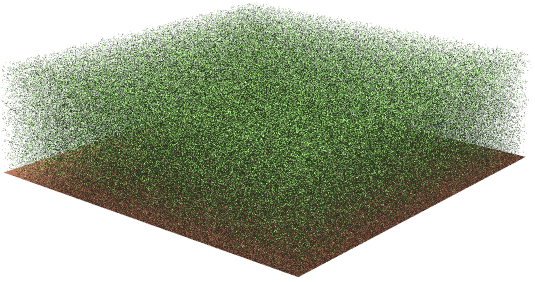
\includegraphics[width=0.5\textwidth]{/home/mn811042/Thesis/chapter2/figures/Figure_1_HOM01.png}
\caption{Structurally homogeneous canopy scenario with infinitesimally small (turbid) foliage representations (from \citet{Widlowski2007}).}
\label{f:homogeneous_canopy}
\end{figure}

The portion of radiation that goes through a vegetation canopy is mostly determined by the amount of vegetated material within the canopy. Firstly defined as the one-sided leaf area per unit ground area \citep{Watson1937}, LAI is a key variable to link structure and function of ecosystems, because:
\begin{enumerate}
\item LAI influences the radiative balance of LSMs. It is used to calculate the amount of intercepted Photosynthetically Active Radiation (PAR, 400-700 nm) by leaves, which is related directly to the amount of CO$_2$ assimilation through photosynthesis \citep{Norman1982,DePury1997}; it is related to the amount of reflected shortwave radiation by the surface \citep{Ni2000,Anderson2005}, which has an impact on the energy balance; and finally, it affects canopy transmittance, that impacts soil temperature and the timing of snowmelt \citep{Hardy1997};
\item rainfall interception \citep{Aston1979}, canopy evapotranspiration \citep{Leuning1995,Baldocchi2002}, and soil evaporation \citep{Schulze1994,Kelliher1995} are also impacted by LAI, and have implications on the hydrological ecosystem dynamics;
\item emissions and depositions of trace gases such as isoprene, NO$_x$ and SO$_x$ \citep{Hicks1987,Baldocchi1999} are also influenced by LAI.
\item it can also interferes with momentum exchanges between the surface and the atmosphere. LAI interferes with a negative feedback by increasing drag on wind, decreasing wind velocity that acts to reduce mass and energy exchange \citep{Albertson2001}.
\end{enumerate}

Determining and understanding LAI appropriately is fundamental to accurately obtain most of the biogeophysical processes in LSMs. Different plant functional types (PFTs) are characterised by different amount and range of LAI, leaf biomass and leaf area density \citep{Asner2003}. Correlative and biogeographical analyses suggested that LAI is strongly tied to site water balance and nutrient status \citep{Woodward1987,Scheffer2005}.

Although the meaning and importance of LAI in radiative transfer formulations are pretty much a consensus, the extinction coefficient has a relatively broad significance, and it is understood as an `open' variable used to attenuate radiation propagation in vegetation canopies, and cannot be explained by the LAI alone.
Several approaches have been proposed to understand and compute extinction coefficient, especially regarding leaf angle distribution \citep{Ross1981}, and different procedures are taken into account for the effect of leaf angle and direction of beam path \citep{Wang2007}. The extinction coefficient can be considered as the fraction of hemi-surface leaf area that is projected onto the horizontal, from a particular zenith angle ($\theta$). In other words, it is possible to equate $k$ to the ratio between the shadow cast by a leaf on the horizontal and the area of the leaf \citep{Monteith1990}.

In real canopies many leaves exist with a statistical distribution of elevation and azimuth angles. The leaf orientation function is derived using solid angle geometry \citep{Ross1981,Myneni1989}, since foliage elements are oriented in various directions in plant canopies, the projected area in one direction does not contain all the information for estimating radiation interception. When the foliage angular distribution is spherical (random), the usual projection coefficient of 0.5 can be used for objects of any shape \citep{Chen1997}, and this value is commonly assigned to $k$ in the literature.

Because of its theoretical simplicity and computational efficiency, the Beer\textsinglequote s law has been used in most LSMs, however, it does not account for the loss of scattered radiation \citep{Wang2003}. Radiative scattering processes are fundamental to accurately determine the Earth\textquotesingle s surface albedo, which is a basic control factor for the surface energy budget \citep{Dickinson1983}. \citet{Charney1975} proposed the biogeophysical feedback theory in the Sahel region that deforestation leads to less surface vegetation, which raises the surface albedo and, in turn, due to changes in the energy balance, the Earth\textquotesingle s surface becomes a radiative heat source. Radiative cooling of the atmosphere over the Sahara due to the enhancement and sustenance of downwelling air leads to the expansion of the desert margins. Later, \citet{Charney1977} supported this earlier hypothesis through experiments with GCMs. Statistical tests have shown that the average atmospheric flow and climate are sensitive to changes in surface albedo, which indicates that the surface albedo is a very important variable in climate models \citep{Dai2007}.

\subsection{The two-stream scheme}\label{sec:2st_scheme}

In order to treat the effects of multiple scattering by cloud particles, aerosols and air molecules, the two-stream approximations are employed in most shortwave radiation (i.e., solar, 300-2500 nm) schemes presently used in LSMs for numerical weather prediction and climate modelling. In two-stream approximations, the radiation field is divided into the direct solar beam, plus the diffuse solar radiation (i.e., radiation scattered at least once), and in two directions, downward and upward fluxes. The angular distribution of scattered radiation is not computed in any further detail, which means they are considered to be isotropic \citep{Raisaenen2002}. 

The two-stream approximation, or scheme has been used to deal with radiative transfer in the atmosphere for many years. The basic procedure in applying it to vegetation is to expand a complex function in the control equations into Legendre functions and then truncate them to the first order closure to get a simple solution \citep{Dai2007}. After reviewing several variants of the two-stream approximation model in the calculation of atmospheric radiation, \citet{Meador1980} presented a unified form of the variants and introduced a new and improved method.

\citet{Dickinson1983} introduced this new two-stream method to estimate radiative transfer in a vegetated canopy, and \citet{Sellers1985} used the two-stream approximation to calculate values of hemispheric canopy reflectance in the visible and near-infrared (NIR) wavelength intervals. The two-stream approximation treatment has been widely used in land surface process models until nowadays.
The approximation assumes that diffuse radiative fluxes are isotropic in the upward and downward directions. Supposing that the upper and lower leaf optical properties are identical, the two-stream approximation used to model radiative transfer in plant canopies is given in the following form \citep{Dickinson1983,Sellers1985}:
\begin{equation}
\begin{gathered}
-\overline{\mu}(dI^{\uparrow})/dL + [1 - (1 - \beta)\omega]I^{\uparrow} - \omega \beta I^{\downarrow} = \omega \overline{\mu} K \beta_0 \exp{(-KL)},\\
-\overline{\mu}(dI^{\downarrow})/dL + [1 - (1 - \beta)\omega]I^{\downarrow} - \omega \beta I^{\uparrow} = \omega \overline{\mu} K (1-\beta_0) \exp{(-KL)}
\end{gathered}
\end{equation}\label{eq:two_stream}
\noindent where $I^{\uparrow}$ and $I^{\downarrow}$ are the upward and downward diffuse radiative fluxes normalized by the incident flux respectively, $\mu$ is the cosine of the zenith angle of the incident beam, $K$ is the optical depth of direct beam per unit leaf area and is equal to $G(\mu)/\mu$, $G(\mu)$ is the relative projected area of leaf elements in the direction $cos^{-1}\mu$, $\overline{\mu}$ is the average inverse diffuse optical depth per unit leaf area and is equal to $\int_{0}^{1}[\mu^{\prime}/G(\mu^{\prime})]d\mu^{\prime}$, $\mu^{\prime}$ is the direction of scattered flux, $\omega$ is the scattering coefficient and is equal to $\rho_{leaf} + \tau_{leaf}$, and $L$ is the cumulative LAI. $\beta$ and $\beta_0$ are upscattering parameters for the diffuse and direct beams respectively (see \citet{Sellers1985} for details). 

Equations~\ref{eq:two_stream} can be solved as an exact solution with appropriate boundary conditions \citep{Sellers1985}. For direct incident radiation, the appropriate top boundary condition is $I^{\downarrow}$ = 0 for L = 0, and the bottom boundary condition is $I^{\uparrow} = \rho_s[I^{\downarrow} + \exp{(-kL_T)}]$ for $L = L_T$, where $\rho_s$ is the soil reflectance and $L_T$ is the total LAI. The corresponding solution of Equations~\ref{eq:two_stream} yields \citep{Sellers1985} are:
\begin{equation}
\begin{gathered}
I^{\uparrow} = \frac{h_1\exp{(-KL)}}{\sigma} + h_2\exp{(-hL)} + h_3\exp{(hL)},\\
I^{\downarrow} = \frac{h_4\exp{(-KL)}}{\sigma} + h_5\exp{(-hL)} + h_6\exp{(hL)}
\end{gathered}
\end{equation}\label{eq:two_stream_dir}
For diffuse radiation, the appropriate top boundary condition is $I^{\downarrow}$ = 1 for L = 0, and the bottom boundary condition is $I^{\uparrow}$ = $\rho_sI^{\downarrow}$ for $L = L_T$. Then, the corresponding solution is given as:
\begin{equation}
\begin{gathered}
I^{\uparrow} = h_7\exp{(-hL)} + h_8\exp{(hL)},\\
I^{\downarrow} = h_9\exp{(-hL)} + h_{10}\exp{(hL)}
\end{gathered}
\end{equation}\label{eq:two_stream_dif}
\noindent where coefficients such as $\sigma$ and h$_1$ to h$_{10}$ are given in \citet{Sellers1985}. Note that there is an error in the expression for h$_4$ in the appendix of \citet{Sellers1985}. The correct expression can be found in \citet{Sellers1996}. %\citep{Dai2007}.

\section{Impacts of using different radiative transfer schemes}

The amount of absorbed radiation obtained with the Beer\textquotesingle s law overestimate the values calculated with the two-stream approximation \citep{Wang2003}. As previously discussed, the Beer\textquotesingle s law does not consider any order of scattering, which implies that by using this method, any interaction between the downward beam radiation and elements of the vegetation canopy is assumed to be absorbed. 

On the other hand, the two-stream approximation considers first order scattering, which means that part of the downward beam radiation after interaction with the vegetation canopy is scattered in an isotropic diffuse form. The upward scattered radiation not absorbed by the vegetation canopy is the sum between the contribution of scattered radiation by the vegetation and the one scattered by the background soil. The scattered radiation by the background soil can either be absorbed by the vegetation canopy, or be transmitted upwards without suffering any further interaction. 

As a result of misrepresenting radiation scattering, Beer\textquotesingle s law has greater amounts of radiation absorption and lower amounts of reflection in comparison to the two-stream approximation. The simplest version of Beer\textquotesingle s law which uses a single exponential function without considering the direct beam and diffuse radiation separately is considered to be too inaccurate for estimating the radiative balance of a plant canopy, and is therefore not indicated to be used \citep{Wang1990a}. 
The development of more complex schemes that explicitly consider more realistic phenomena in radiative transfer models was only possible with the advent of new technologies, e.g. more computational power, acquisition of new data, which the satellite era allowed more available radiometric products to be used in LSMs calculations; and the proposition of new theories and methods, with the development of 3D radiative transfer models \citep{Wang1990} was possible to establishes important misrepresentations in the radiative balance by simpler models. 
%The impacts of using either Beer\textquotesingle s law, or two-stream to estimate the radiative transfer in vegetation canopies was investigated by several authors and are briefly explored in the following section.

In a sensitivity analysis performed by \citet{Alton2007} using measured meteorological and flux data for three different ecosystem (boreal, tropical, and temperate forests), the differences between measured and simulated gross primary productivity (GPP) were evaluated for different radiative transfer schemes available in the JULES (Joint UK Land Environment Simulator) model \citep{Best2011,Clark2011}, whose Beer\textquotesingle s law and the two-stream approximation are included. 

In JULES, GPP is calculated by a modified version of the Farquhar model \citep{Farquhar1980,Collatz1991,Collatz1992}, where leaf photosynthesis is dependent on a number of environmental variables as well as the internal CO$_2$ concentration. Figure~\ref{f:gpp_difference_beers} shows differences in GPP between the two-stream approximation and Beer\textquotesingle s law. The authors obtained values for global GPP derived with Beer\textquotesingle s law and with the two-stream approximation equal 131 Gt and 129 Gt, respectively. The authors also pointed out that the major differences were founded in regions with higher mean LAI. For example, GPP predicted by Beer\textquotesingle s law for the tropics was up to 25\% higher than equivalent output from the two-stream approximation. 

The two-stream method used in this comparison exercise followed the multilayer approach including sunlit and shaded leaves parameterisation with nitrogen profile decreasing vertically through canopy, and inhibition of leaf respiration in light \citep{Mercado2007}. The differentiation between sunlit and shaded leaves, or the `sunfleck penetration' \citep{Dai2004} was an attempt to account for direct light penetration into the vegetation canopy, and the better agreement of this scheme with observed data, in comparison to Beer\textquotesingle s law, is an indicator of the importance of considering vegetation canopy as being irregular, i.e., places with no vegetation at all, that allows direct solar radiation penetrates the vegetation canopy without being scattered, and other places with vegetation.
%In other words, the parameterisation proposed by \citet{Mercado2007} tried to account for a natural clumped vegetation.

\begin{figure}[ht!]
\centering
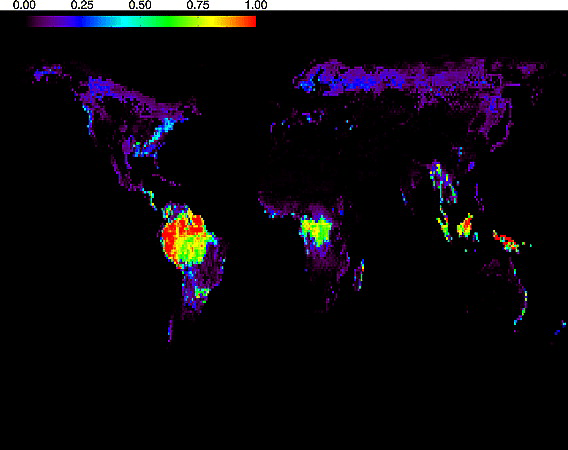
\includegraphics[width=0.5\textwidth]{/home/mn811042/Thesis/chapter2/figures/Figure_2_alton_2007.png}
\caption{Beer\textquotesingle s law and the two-stream schemes difference in GPP (kgm$^{-2}$yr$^{-1}$) predicted by JULES with two different representations of radiative transfer in the canopy. The colour table is scaled from 0.0 (black) to 1.0 kgm$^{-2}$yr$^{-1}$ (red) (from \citet{Alton2007}).}
\label{f:gpp_difference_beers}
\end{figure}

Another study based on the evaluation of differences between radiative transfer schemes present in LSMs can be found in \citet{Huntingford2008}. The authors performed a sensitivity study between Beer\textquotesingle s law and a modified version of two-stream approximation with the same introduction of a more realistic depiction of light levels within a vegetation canopy \citep{Jogireddy2006,Mercado2007} in order to quantify uncertainties in predictions of Amazon ``dieback'' \citep{Cox2000}. 

The authors used the MOSES \citep{Cox1999} model and calculated its effect on stomatal conductance, and thus control on photosynthesis, and evaporation to determine the impact on modelled vegetation and soil carbon, for the Amazon rainforest during the twenty-first century. In a multilayer approach, absorption and scattering losses of incident radiation, for both direct and diffuse radiation, were calculated at different levels in the canopy. These included contributions from the visible and near infrared (NIR, 700-1000 nm) wavebands.

The improved light interception model has been successfully tested against eddy correlation measurements for a rainforest site in Manaus \citep{Mercado2007}. The authors found that the main improvement of introducing the `two-stream/multilayer' description was to allow a more realistic modelling of the response of photosynthesis to light, and the associated impact on the diurnal cycle of modelled carbon and water fluxes \citep{Huntingford2008}. 

The authors explained that the MOSES-modelled photosynthesis tended to saturate quickly for increasing solar radiation, generating a `flat' response in the middle of the day, whereas measurements indicate photosynthetic response to varying light levels for the entire diurnal period. The introduced scheme simulated higher GPP, but lower net primary production, and thus lower plant and soil carbon pools relative to the original Beer\textquotesingle s law simulation (Figure~\ref{f:huntingford2008}). 

The authors identified the improved treatment of radiation absorption as having little alteration to the original dieback result obtained with the standard radiation scheme, however the future simulations of vegetation carbon and soil carbon seemed to be approximately 25\% smaller when using the two-stream approximation, instead of using Beer\textquotesingle s law. 

\begin{figure}[ht!]
\centering
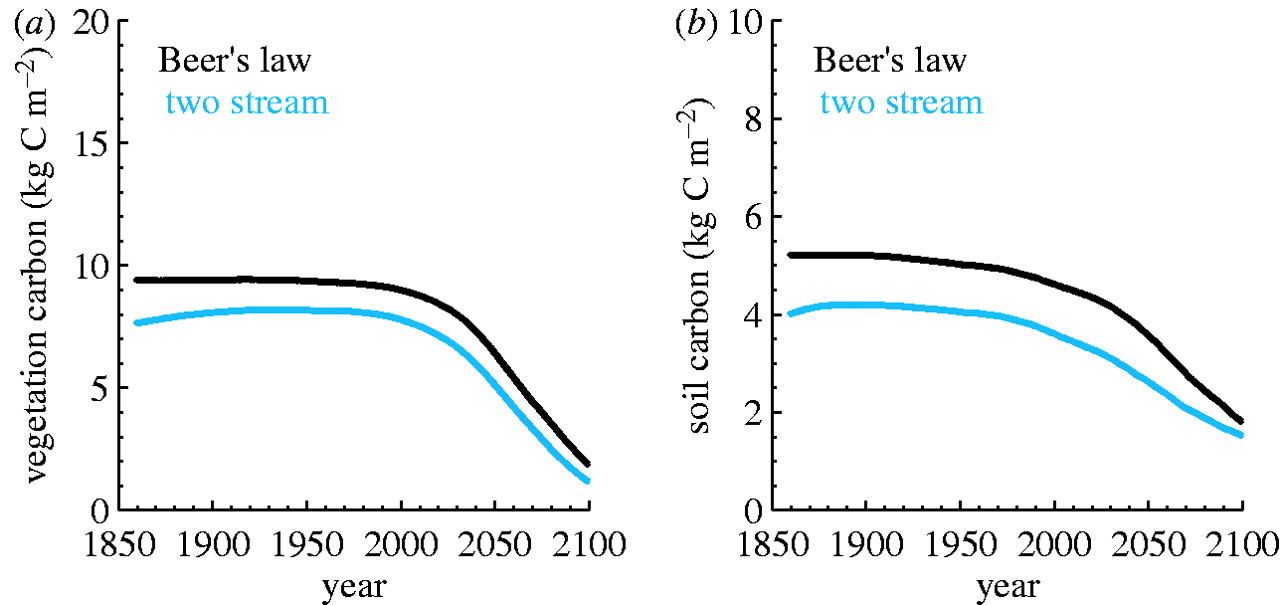
\includegraphics[width=1.0\textwidth]{/home/mn811042/Thesis/chapter2/figures/Figure_3_huntingford_2008.png}
\caption{Changes in Amazonian (a) vegetation and (b) soil carbon for the Amazon region using climate change patterns derived from the original \citet{Cox2000} simulation. The black curve corresponds to the standard `big-leaf' version of the land surface scheme and the blue curve the review `two-stream' approach to light interception (from \citep{Huntingford2008}).}
\label{f:huntingford2008}
\end{figure}

The study of \citet{Huntingford2008} noted a negative impact on carbon storage when using a more ``transparent'' vegetation canopy to solar radiation by including: (i) spectral properties of the vegetation canopy and background soil (e.g. leaf reflectance, transmittance and background soil albedo), (ii) differences in the nature of light (e.g., different mathematical formulation for direct and diffuse light), and (iii) an irregular canopy (e.g., different mathematical formulation for sunlit and shaded leaves). 
By considering an irregular canopy, or canopy structure, the inclusion of canopy heterogeneities in different radiative transfer schemes in LSMs achieved an impact of up to 30\% on GPP in another study \citep{Alton2007}.

These comparative studies were focused on testing different radiative transfer schemes broadly used in LSMs, and somehow to evaluate the performance of a new parameterisation for canopy sunlit/shaded leaves \citep{Mercado2007}. Their results indicated a strong evidence that canopy structural heterogeneity impacts carbon assimilation and balance. They also noted that these impacts are important to improve the understanding of the complex radiative transfer phenomenon, and reduce uncertainties in LSMs predictability of diagnostic variables that will impact climate predictions.

Several authors \citep{Nilson1971,Chen1997,Kucharik1999,pinty2006,Ni-Meister2010} attempted to address canopy heterogeneities in a simple way to be directly used in LSMs. Their attempt in producing something ``simple'' are related to (i) computational efficiency, and (ii) availability of input parameters.

In \citet{Yang2001} a complex 3D radiative transfer model was tested against the two-stream approximation and results indicated that a factor of roughly 50 times more CPU time was required for the complex model, depending on the vertical resolution used. The authors concluded that the inclusion of a complex 3D model with such an elevated CPU demand in LSMs was not plausible. Also, it was well known before, that vegetation canopy architecture could affect radiation propagation \citep{Nilson1971}, however, a lack of observational data led to inaccuracies in specifying model parameters, such as between and within-crown gaps, needle-to-shoot clumping, and forest stand density. 

Even though one of the aims of large scale experiments, such as FIFE \citep{Hall1995}, BOREAS \citep{Sellers1997}, LBA \citep{Keller2004} was to improve and validate parameterisations, and to enhance methods for deriving parameter from fieldwork observations, they were limited in space and time, therefore not suitable for global applications in GCMs, for example. 
The next section describes the first theory considering canopy structure in radiative schemes in a simple manner, evaluates proposed parameterisations pointing out their pros and cons, and discusses possible ways to address these problems in this thesis.

\section{Considering vegetation canopy structure in radiative transfer schemes}

In both schemes evaluated previously (Beer\textquotesingle s law vs. two-stream approximation), the representation of vegetation has been as homogeneous canopies of single vegetation types, which might or might not include mosaicked cover types to represent heterogeneities in LSMs. 

Efforts have been made in order to consider vegetation architectural irregularities in radiative transfer schemes, as the sunlit/shaded leaves parameterisation developed by \citet{Mercado2007}, for example, however, their treatment of different properties of incident light (diffuse-shaded vs. direct-sunlit) in vegetation canopies does not directly account for vegetation structure itself. It is known that the amount of radiation absorbed, reflected, and transmitted in plant canopies depends on the beam fraction of incident radiation, the optical properties of the plant elements, the albedo of the underlying soil/snow surface and canopy structure \citep{Ross1981}. 

For most natural woody vegetation, such as conifer forests, deciduous forest, savannah/woodland/shrubland, various sizes of gaps exist between different tree crowns, the term `gaps' is used here in the sense of `openness', i.e., canopy openings, which light goes through unintercepted to the point of observation. Using the two-stream approximation can result in errors when estimating PAR absorption, surface albedo and other radiative fluxes such as longwave radiation for canopy leaf temperature estimates \citep{Ni-Meister2010}. 

Canopy structure is generally understood as the spatial and temporal arrangement of forest components, or canopy elements, at various scales. The geometric approach to canopy structure seeks to quantify the area, pattern and orientation of organs such as leaves, trunks, flowers and fruits, and the size, morphology and dispersion of gaps which separate them \citep{Ross1981,Norman1989}. Canopy gaps are useful measures for remote sensed vegetation analyses, for monitoring phenological changes, plant recovery after environmental impact and stress, canopy dynamics, throughfall and effects of air pollution or pest outbreak on foliage denseness \citep{Walter2012}. 

Observations of canopy gaps and detailed geometric models demonstrate that clumping of vegetation and foliage is a significant factor affecting the vertical light profile in many canopies, such as needle-leaf forest, savannahs and, in general, in forest canopies that are not completely closed \citep{Nilson1971,Kucharik1999,Yang2001,Jonckheere2004,Chen2008,Ni-Meister2010}.

Foliage clumping has been shown to be significant for accurate calculation of albedo \citep{Ni2000}, absorbed PAR \citep{Chen2008}, photosynthesis \citep{Law2001}, the vegetation energy balance \citep{Anderson2005}, and the timing of snowmelt \citep{Hardy1997}.

To characterise the spatial clumping of vegetation structure on radiation regime, \citet{Nilson1971} introduced a clumping factor, $\Omega$($\theta$), into Beer\textquotesingle s law in order to characterise the plant canopy direct transmittance, or gap fraction, P$_{gap}$:
\begin{equation}
 P_{gap}(\theta) = \exp{(\frac{-G(\theta)LAI\Omega(\theta)}{cos\theta})}
\end{equation}\label{eq:pgap}
\noindent where $\theta$ is the Sun zenith angle, and $G$($\theta$) is the leaf angle distribution, which is the projection coefficient of unit foliage area on a plane perpendicular to the view direction \citep{Ross1981}, as previously discussed. When $\Omega$($\theta$) = 1, there is no clumping and leaves are considered to be randomly distributed. When $\Omega$($\theta$) $<$ 1, the beam transmission is enhanced by clumping, which usually is the case in most of clumped vegetation canopies. But it is also possible to have cases where $\Omega$($\theta$) $>$ 1, then the formulation can be interpreted as the beam transmittance is decreased by canopy clumping effects.
The clumping index quantifies the spatial distribution pattern of leaves \citep{Norman1974}, and it has been usually quantified based on gap size distribution measured from Tracing Radiation and Architecture of Canopies instrument (TRAC; 3rd Wave Engineering, ON, Canada) \citep{Leblanc2002} or digital hemispherical photographs \citep{ChenandCihlar1995,Leblanc2005}. 

Main challenges to correctly quantify and interpret $\Omega$($\theta$) in forests include the range of view zenith angles, the type of calculation methods, and how $\Omega$($\theta$) changes with $\theta$ \citep{Ryu2010}. Several authors have shown the variance of $\Omega$($\theta$) with $\theta$ \citep{Andrieu1993,Chen1996,Kucharik1999,Chen2008}, and angular dependence of clumping is an important characteristic to determine spatially representative $\Omega$($\theta$). 

The underlying mechanism of clumping varying with Sun zenith angles remains unclear. Previous studies from several boreal needle-leaved forest report that clumping index increased with zenith angle \citep{Chen1996,Kucharik1999}. However, in a more recent study, \citet{Ryu2010} found an opposite behaviour for clumping index varying with zenith angle, i.e., decreased with Sun zenith angle, when analysing a heterogeneous savannah. The authors suggested that when canopies are horizontally dense and vertically prolonged, the path length of a ray through the canopies increases with zenith angle. Longer path lengths make large gaps be decomposed into smaller ones, which is closer to random gap size distribution. They suggested that the angular dependence of clumping index was controlled by ecosystem scale tree distribution patters to some degree, and it might be a unique characteristic in heterogeneous savannahs ecosystem, specifically a blue oak woody savannah in their study. 

Some authors attempted to formulate simplified modelling approaches to resolve vegetation clumping at several levels of organisation, in order to address one major difficulty associated with radiative transfer in forest canopies. From now on, this section will discuss what has been found and their results.

The first study evaluated in this section was developed by \citet{Kucharik1999}. The authors used measurements of LAI and gap fraction made with MVI (Multiband Vegetation Imager) \citep{Kucharik1997} obtained during BOREAS \citep{Sellers1997} field campaigns of 1994-1996 to derive a semi-empirical \citep{Ni-Meister2010} relationship between $\Omega(\theta)$ and zenith angle ($\theta$). In this method, two key quantities are needed: (i) the fraction of ground area covered by the horizontal projection of crown envelopes (f$_c$) (from nadir view), which is a function of the typical tree crown diameter ($D$), and tree stem spacing ($\lambda$), or stem density, within a study plot; and (ii) an estimate of crown porosity ($\Phi$); this quantity is related to foliage density and defined as the gap fraction within crown envelopes divided by f$_c$.

A series of zenith gap fraction measurements were needed along a transect beneath a canopy to partition the total gap fraction ($f_{gap},t(0)$) between within-crown and between-crown gaps, and  an estimate of the total fraction of ground area covered by the horizontal projection of crown envelopes ($f_c$). To obtain $f_c$, the typical crown silhouette area ($\pi R^2$, where $R$ is the crown radius in the horizontal direction) is multiplied by the number of crowns and divided by the total ground unit area on which the stem density is based. If $f_c$ is greater than 1, crowns typically overlap in the forest, and the entire value of $f_{gap},t(0)$ can be defined as within-crown gap fraction ($f_{gap},c(0)$). The total gap fraction occurring between-crowns ($f_{gap},b(0)$) can be estimated by $1 - f_c$, and $f_{gap},c(0)$ is therefore approximated by $f_{gap},t(0) - f_{gap},b(0)$. If the value of $f_{gap},c(0) < 0$, it can be assigned a value of 0 for all practical purposes. 

Crown porosity ($\Phi$) is determined by dividing $f_{gap},c(0)$ by $f_c$ ($\Phi$ = $f_{gap},c(0)/f_c$). The value of $\Phi$ may be described as a normalised within-crown gap fraction. Generally, an error of about 0.05 exists in determining $f_c$ and $\Phi$ by using an average crown radius and tree stem density rather than the actual model calculations of $f_c$. However, the authors indicated that these errors are not of concern when estimating $\Omega(0)$ using the gap-fraction partitioning strategy.

Values of $\Phi$ and $f_c$ were then used to determine a value of $\Omega$(0) that was consistent with calculations resulting from numerical simulations of the canopy gap-size distribution. A non-linear least-squares fit to approximately 250 Monte Carlo simulations (analysing values of $\Omega(0)$) was performed for values of $f_c$ $\geq$ 0.20, and for all simulated values of $\Phi$. A separate fit to the entire set of model data was performed for 0.04 $\geq f_c \geq$ 0.30. For sparse canopies where $f_c < 0.20$, a value of $\Omega(0)$ could still be determined. 

Ten equations were solved simultaneously to determine 10 coefficients ($a_0$, ..., $a_9$) that describe the relationship between values of $\Omega(0)$, $f_c$, and $\Phi$. To characterise the angular dependence of $\Omega(\theta)$, a minimum value of $\Omega(\theta)$ was determined at $\theta$ = 0$^{\circ}$ and a value of $\Omega(\theta)$ was needed at $\theta$ = 90$^{\circ}$. Because it was assumed that $\Omega(\theta)$ reaches its maximum value at $\theta$ = 90$^{\circ}$, \citet{Kucharik1999} refer to this value as the maximum possible element clumping index, $\Omega_{max}$, and defines it as:
\begin{equation}
\Omega_{max} = \Big(\frac{ND}{\sqrt{A}}\Big)^{0.7}
\label{equation:clumpmax}
\end{equation}
\noindent where $N$ is number of stems within ground area $A$, and $D$ is crown diameter. If $ND/\sqrt{A} > 1$, then the value of $\Omega_{max} = 1$. The angular dependence of $\Omega(\theta)$ was defined by \citet{Kucharik1999} following the equation: 
\begin{equation}
\Omega = \Omega(\theta) = \frac{\Omega_{max}}{[1 + b\exp(-k(\theta)^p)]}
\end{equation}\label{equation:clumptheta}
\noindent where $k$ is constant (usually $k$ = 2.2), $\theta$ is zenith angle expressed in radians, and $b$ is solved from a rearrangement of Eq.~\ref{equation:clumptheta} using a known value of $\Omega(\theta)$ (e.g., $\theta$ = 0$^{\circ}$). A quantitative comparison of results produced using Eq.~\ref{equation:clumptheta} with the best-fit curves suggested that a value for $p$ can be approximated by an equation on the form:
\begin{equation}
p = -0.461\chi + 3.8
\label{equation:pchi}
\end{equation}
\noindent where $\chi$ is the ratio of crown depth to crown diameter. Generally, if $\chi$ is $\leq$ 1.0, $p$ = 3.34. 

\citet{Kucharik1999} used this set of semi-empirical equations to estimate clumping index for five different forest types: jack pine, black spruce, aspen, oak and sugar maple. The results calculated by Eq.~\ref{equation:clumptheta} are presented by dashed lines in Figure~\ref{f:kucharik}. The authors also presented the best fit to data for each forest site by solid lines in the same figure. The range of clumping index obtained by this work was from approximately 0.37, for minimum Sun zenith angle (i.e., $\theta$ = 0$^{\circ}$), with convergence to 1, for maximum Sun zenith angle (i.e., $\theta$ = 90$^{\circ}$).

\begin{figure}[ht!]
\centering
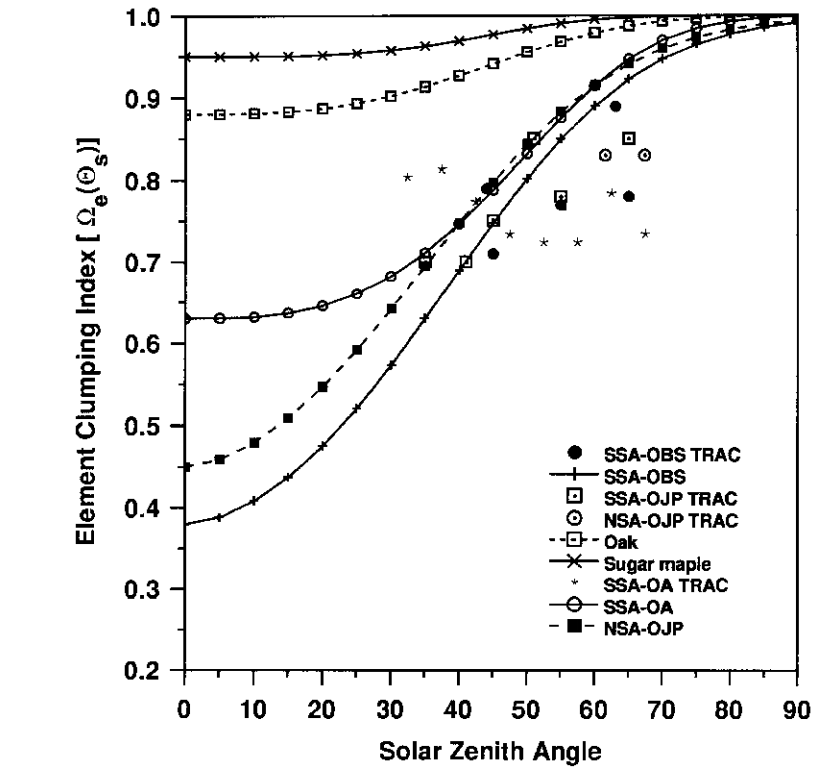
\includegraphics[width=0.5\textwidth]{/home/mn811042/Thesis/chapter2/figures/Figure_4_kucharik_1999.png}
\caption{Results of general solution of $\Omega(\theta)$ calculated by Eq.~\ref{equation:clumptheta} with independent values of $\chi$ and p for the five forest species. Dashed lines represent the result of Eq.~\ref{equation:clumptheta} with k = 2.2 and p = 3.0 for aspen, p = 3.34 for sugar maple and oak, p = 2.19 for jack pine, and p = 1.50 for black spruce. Solid lines represent the best fit to data for each forest (from \citet{Kucharik1999}).}
\label{f:kucharik}
\end{figure}

\citet{Kucharik1999} showed the behaviour of clumping index increasing with Sun zenith angle for all evaluated sites in this study. It is also possible to distinguish between three groups of clumping index: a high varying clumping index observed for black pine and jack spruce, both needle-leaved species; a medium varying clumping index for aspen; and a low varying clumping index for oak and sugar maple; the last tree broad-leaved species. 

The semi-empirical relationship underestimated the best-fit clumping index for jack pine over all Sun zenith angles, and overestimated the best-fit clumping index for aspen for Sun zenith angles higher than 20$^{\circ}$. For the other cases, the adjust presented a fair agreement of clumping index.

Following the same attempt to derive a relationship for clumping index, \citet{Ni-Meister2010} developed an analytical prognostic expression based on stem density ($\lambda$), crown radius ($R$) and LAI. In here, only the equation used for spherical crowns is shown, however, the same authors extend the analysis to more generalised ellipsoid crowns, as introduced in \citet{Li1988}. The analytical solution for the modified clumping index in Beer$^{\prime}$s law is expressed as, 
\begin{equation}
\Omega = \gamma = \frac{3}{4\tau_0R}\Big(1 - \frac{1 - (2\tau_0R + 1)\exp(-2\tau_0R)}{2\tau_0^2R^2}\Big)
\label{equation:clumpNi}
\end{equation}
\noindent where $\tau_0r = 3 G LAI/ 4 \lambda \pi \cdot R^2$ for spherical crowns.

The authors compared the analytical solutions for clumping factor with the ones calculated by the full GORT model \citep{Li1995}, which was specifically developed to describe the effects of 3D canopy structure on the radiative balance and to characterise the heterogeneous radiative balance in natural vegetation at the forest stand scale. 
To analyse the difference in clumping index estimated by the analytical and full GORT models, Figure 5 compares the two models for 32 deciduous plots in Harvard Forest, MA \citep{Barford2001}. Only tree height and diameter at breast height (DBH) were actually measured, while the rest of GORT input parameters were calculated based on allometric equations \citep{Ni-Meister2010}. Changes in clumping index with different structure parameters shown very similar patterns for the analytical and full GORT models. 

\begin{figure}[ht!]
\centering
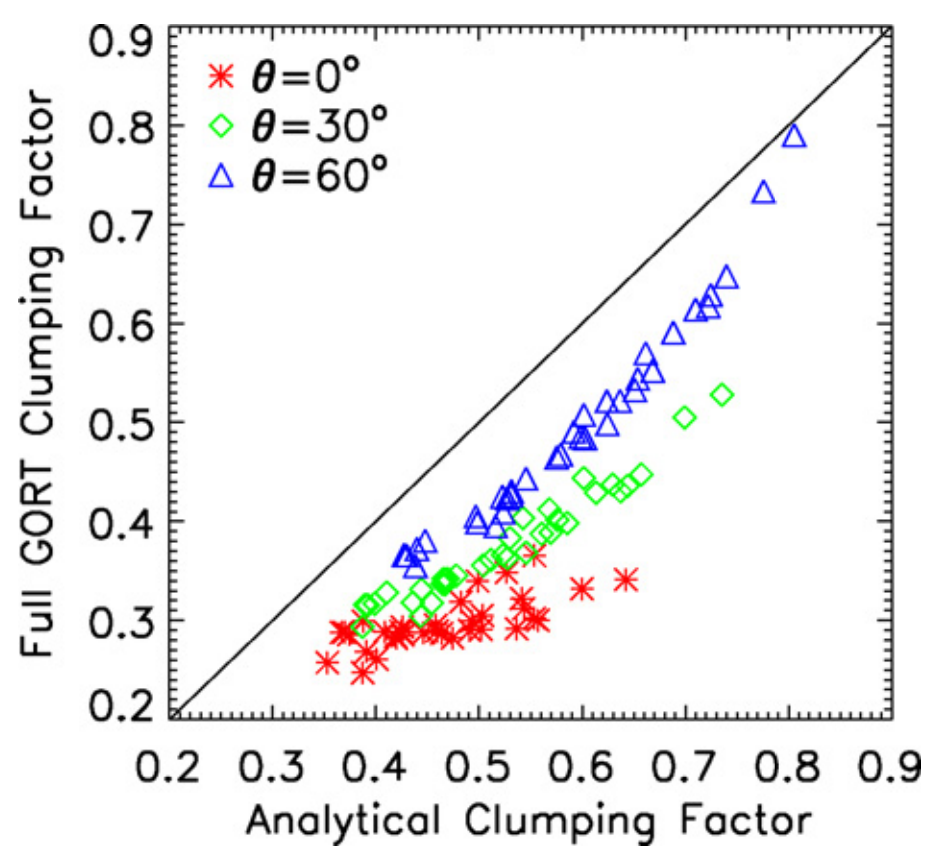
\includegraphics[width=0.5\textwidth]{/home/mn811042/Thesis/chapter2/figures/Figure_5_ni_meister_2010.png}
\caption{Comparison of clumping factors calculated from the full GORT and analytical GORT models for 32 deciduous plots in Harvard Forest, MA (from \citet{Ni-Meister2010}).}
\label{f:ni-meister}
\end{figure}

The analytical clumping factor is larger than the full GORT modelled values, because the full GORT assumption of random crown distributions results in over-clumping. The analytical clumping factor is always larger  less clumped  since it takes into account the condition that tree crowns do not overlap. The difference becomes smaller at larger solar zenith angles \citep{Ni-Meister2010}.

Differently than the previous parameterisation, \citet{Ni-Meister2010} evaluated their analytical clumping index in relationship to a more complex 3D radiative transfer model instead of observed data. This exercise allowed the authors to build a perfectly controlled experimental scenario in a modelling experiment, and evaluate changes in clumping index with different structure parameters such as tree density, horizontal crown radius, foliage density and vertical/horizontal crown radius ratio. Their results shown agreement with the previous parameterisation and their conclusion is that clumping index increased with Sun zenith angle for all evaluated scenarios independently of canopy structure. They also shown extra results regarding canopy structure. 

In their modelling experiment, clumping index increased with tree density and vertical/horizontal crown radius ratio, which means that dense vegetation canopies (e.g. tropical forest), and tall trees (e.g., sequoias) approximates the radiative transfer to the random case, i.e., $\Omega(\theta)$ = 1. 

Their second finding, related to canopy structure, is that clumping index decreased with horizontal crown radius and foliage density. The authors did not explained exactly why and how, but a preliminary explanation is proposed in here. By increasing horizontal crown radius and keeping everything else constant (i.e., tree density, foliage density and vertical/horizontal crown radius ratio), there are an increasing in number and size of within-crown gaps, which turns the vegetation canopy more heterogeneous, more ``gappy'' as a whole. On the other hand, by increasing foliage density, there are a decreasing of within-crown gaps, turning the canopy less gappy as a whole, but increasing the ratio between-crown gaps/total gaps. \citet{Ryu2010} indicated a relationship between canopy cover and between-crown gaps/total gaps ratio as being inversely proportional, i.e., if a vegetation canopy presents a high between-crown gaps/total gaps ratio, it is somehow equivalent of being a sparser canopy, with lower tree density (Figure~\ref{f:ryu2010}). These explanations still need further investigations.

\begin{figure}[ht!]
\centering
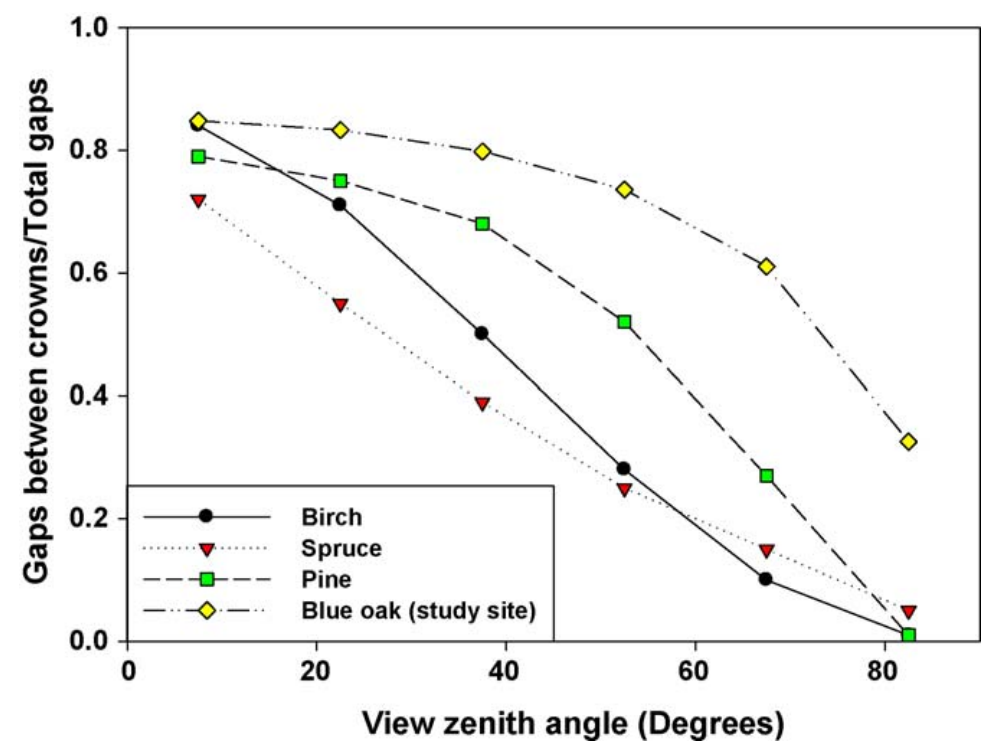
\includegraphics[width=0.5\textwidth]{/home/mn811042/Thesis/chapter2/figures/Figure_6_ryu_2010.png}
\caption{The ratio of gaps between crowns to total gaps among four tree species simulated by \citet{Nilson1999} model. Canopy covers were 0.80, 0.90, 0.74 and 0.47 for birch, spruce, pine and blue oak, respectively. Data source of birch, spruce and pine is \citet{Nilson1999} (from \citet{Ryu2010}).}
\label{f:ryu2010}
\end{figure}

Quantifying and understanding canopy structure in remote sensing derived products is a current area also being highly explored. Algorithms are developed and implemented in the operational ground segments of Space Agencies (e.g., European Space Agency and the U.S. National Aeronautics and Space Administration) to derive higher level products describing the properties of components of the geophysical system, such as the albedo of land surfaces \citep{Schaaf2002}, the fAPAR \citep{Gobron1999}, and the LAI \citep{Myneni2002}. LSMs should thus periodically ingest these operational products to update the corresponding boundary conditions. However, radiative fluxes and state variables retrieved from remote sensing are not directly useful for GCMs \citep{pinty2006}. 
The most advanced representation of terrestrial surface processes in climate models is confined to simplistic modules implementing 1D (vertical) exchange models, in particular with respect to the transfer of radiation. The radiation component of these 1D modules relies on solutions derived from two-stream approximations \citep{pinty2006}. 

The two-stream formulations thus have to be adapted to represent, at least in simplified forms, the effects of these complexities. In some instances, the proposed solutions require the strict equality between the reflectance and the transmittance of leaves, and are accurate only for leaves with spherical distribution \citep{Sellers1985}. The nature of the physical problem to be solved in that instance fully justifies using such 3D instead of simpler 1D models \citep{Knyazikhin1998a,Widlowski2001,pinty2006}.

\citet{Pinty2004} proposed a parameterisation to the estimation of the radiative balance at the satellite pixel resolution through the use of effective (instead of true) variable values and showed that the same principle applies to all state variables of the radiation transfer problem if one is to ensure the correct radiative balance. For example, the values of effective LAI appropriate for 1D models should be smaller than the true values by a factor varying from 0.3 for sparse to 0.8 for dense forest canopies. The authors showed in Figure~\ref{f:pinty2006} the relationship between true and effective LAI to be expected over a wide range of modelled coniferous forest conditions with BOREAS data \citep{Widlowski2004}. The effective LAI values were estimated using the procedure described in \citep{Pinty2004} and the radiation directly transmitted to the ground was calculated using the Raytran ray tracing Monte-Carlo model \citep{Govaerts1998}.

This parameterisation called ``structure factor'', firstly described in \citep{Pinty2004}, and further discussed and evaluated in \citep{pinty2006}, can be interpreted as being a LAI modifying factor. The structure factor is a smooth function of the Sun zenith angle and, for randomly dispersed aggregation of leaves, i.e., tree crowns, its effect is somewhat analogous to the clumping factor \citep{Nilson1971}, also evaluated and parameterised by \citet{Kucharik1999} and \citet{Ni-Meister2010}.

The need to account for such 3D induced effects thus introduces an additional information parameterising the internal variability of the LAI into the 1D representation of the radiation transfer problem. The values of the effective variables are estimated by inverting a 1D radiative transfer schemes against solutions for the radiative transfer equations generated by a more complex 3D model, or directly to observations. 

\citet{pinty2006} affirmed that the structure factor parameterisation constitutes a very robust approach since it guarantees accurate simulations for all components of the radiative balance (absorptance, reflectance, and transmittance) when using, in direct mode, these effective values, and it does not require an explicit description and understanding of the complex phenomena arising from the presence of heterogeneous vegetation architecture. 

\begin{figure}[ht!]
\centering
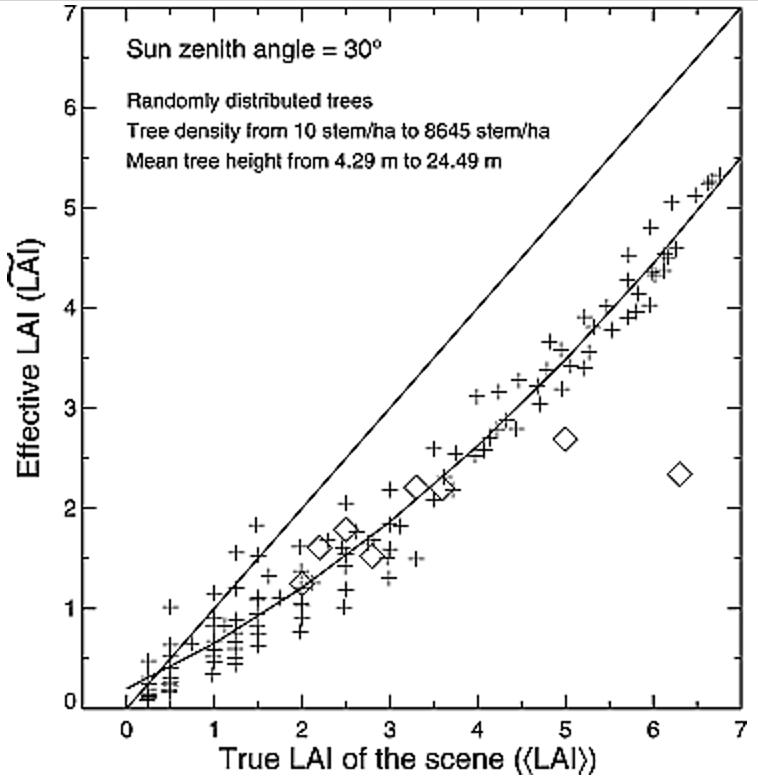
\includegraphics[width=0.5\textwidth]{/home/mn811042/Thesis/chapter2/figures/Figure_7_pinty_2006.png}
\caption{Simulated relationship between true and effective LAI values over a wide range of coniferous forest type taken from \citet{Widlowski2004}. Field measured (diamonds) values, are taken from the BOREAS experiment after \citet{Chen1997a} (from \citet{pinty2006}).}
\label{f:pinty2006}
\end{figure}

By modifying Beer\textquotesingle s law, the structure factor parameter ($\zeta(\mu)$) is placed exactly in the same way the clumping index ($\Omega(\theta)$) was in Eq.~\ref{eq:pgap}, and it modifies the product of LAI, G-function \citep{Ross1981} and the cos$\theta$, associated with the radiation path length:
\begin{equation}
P_{gap}(\mu) = exp{(\frac{-G(\mu)\cdot \zeta(\mu) \cdot LAI}{\mu})}
\label{equation:pgappinty}
\end{equation}
\noindent where $\mu$ is the cosine of Sun zenith angle. Eq.~\ref{equation:pgappinty} suggests the dependency of the structure factor with respect to the cosine of Sun zenith angle and can be approximated by a linear relationship:
\begin{equation}
\zeta(\mu) \approx a + b \cdot (1 - \mu)
\label{equation:structurefactor}
\end{equation}
\noindent where $a$ = $\zeta(\mu=1)$ is the parameter corresponding to an overhead Sun, and $b$ the parameter responsible for include the effects of a range of different Sun geometries. Both parameters are used to account for vegetation canopy heterogeneities and correctly simulate the radiation path length. 

Between the three cited parameterisations, the one proposed by \citet{pinty2006} presents a relatively ``self-sufficiency'', because it does not require any previous knowledge about vegetation structure, and because of that, it can be applied to any vegetation canopy. Each one of the previously discussed parameterisations presents pros and cons that need to be further discussed. 

By following \citet{Kucharik1999}, it is necessary to know the number of stems within a pre-determined ground area, the crown diameter, and the ratio of crown depth to crown diameter. Besides that, Kucharik\textquotesingle s relationship for determining clumping index is a semi-empirical equation adjusted for a specific set of data collected in boreal forests during the BOREAS large experiment. Its applicability could not necessarily be extended to other PFTs.

While in \citet{Ni-Meister2010},  the relationship for clumping index is based on an analytical prognostic expression, which can also just be determined with previous knowledge about stem density, crown radius and LAI. Besides that, the generalised equation for spheres does not depend on Sun zenith angle, which can introduce errors as previously discussed. 

With the structure factor parameterisation, there is no need to have previous knowledge about canopy structure, whereas the parameters are minimised against calculated/measured terms of the radiative transfer equations (absorptance, reflectance, and/or transmittance). However, further investigations need to be done in order to address the parameters variability over different sized areas, different spectral and structural properties.

Therefore this area has been surprisingly neglected until recently, the need for the development of physically consistent radiative transfer schemes in LSMs were highlighted by recent studies (e.g., \citet{Widlowski2011,loew2014}). 

From this section it is possible to summarise that \citet{Kucharik1999} remarkably derived an expression for clumping index based on fieldwork observations, but for a limited area of study. \citet{Ni-Meister2010} derived an analytical solution for clumping index based on more complex 3D radiative transfer models, but there is still a lack of validation studies with observed data. Last, \citet{pinty2006} proposed a straightforward approach that does not need previous information about the vegetation canopy structure itself, but it needs more detailed comparison with 3D radiative transfer models and further fieldwork validation.

\section{A way forward for vegetation canopy structure representation}

Developing LSMs requires prioritisation of resources between different model components, because recent models become more and more complex, for example by incorporating complex carbon fluxes and nutrient cycling. In the past, a lot of attention has been devoted towards an improvement of the biochemical components in LSMs \citep{Goll2012}, whereas biophysical components, like the vegetation canopy radiative transfer, have been neglected because few studies had analysed systematically the major caveats of existing schemes so far \citep{loew2014}. 

There is a current need to assess the consistency and accuracy of radiative transfer schemes in LSMs and to assess the potential impact of uncertainties in the widely used radiative transfer models on surface energy fluxes and carbon production estimates \citep{loew2014}. Testing model results is always a challenge, especially when the model is designed to focus on details, and such assessment requires physically consistent 3D radiative transfer formulations as a reference, for example the radiative transfer models have been tested by the model intercomparison approach \citep{Pinty2001,Pinty2004,Widlowski2007,Widlowski2011,Widlowski2013}, or by different sources of field data, such as bidirectional reflectance \citep{North1996} and transmittance measurements \citep{Wang1990,Law2001,Kobayashi2012}. It is valuable to highlight in here an important experiment particularly design to address differences between radiative transfer schemes of commonly used LSMs. The RAMI4PILPS \citep{Widlowski2011} suite of virtual experiments was designed to evaluate the accuracy and consistency of shortwave radiative transfer formulations under perfectly controlled experimental conditions. More specifically, RAMI4PILPS prescribed a series of virtual canopy scenarios having accurately described structural, spectral and illumination-related characteristics. For these test cases, radiative transfer model simulations have been generated as a reference using a Monte Carlo approach. The Monte Carlo model in question had been extensively verified during previous RAMI phases \citep{Widlowski2007}. Models participating in the RAMI4PILPS had to simulate the canopy albedo, transmission, and absorption in both the PAR and NIR spectral domains. 

Contrary to efforts comparing model simulations against in-situ observations at specific test sites, the RAMI4PILPS approach eliminated uncertainties arising from incomplete or erroneous knowledge of the (i) structural, spectral, and illumination-related characteristics of the canopy target, and (ii) the uncertainties introduced into the reference solution by calibration, sampling and upscaling errors. 

RAMI4PILPS proposed a heterogeneous canopy scenarios where tree crowns were approximated by woodless spheres, so-called an open forest canopy scene, with pre-described size of spheres, the height of the canopy, and the degree of mutual shading between neighbouring crowns (Figure~\ref{f:rami}). For each scenario, simulations for different leaf areas and varying soil brightness were performed, assuming direct incident radiation for three different Sun zenith angles as well as isotropic illumination conditions.

\begin{figure}[ht!]
\centering
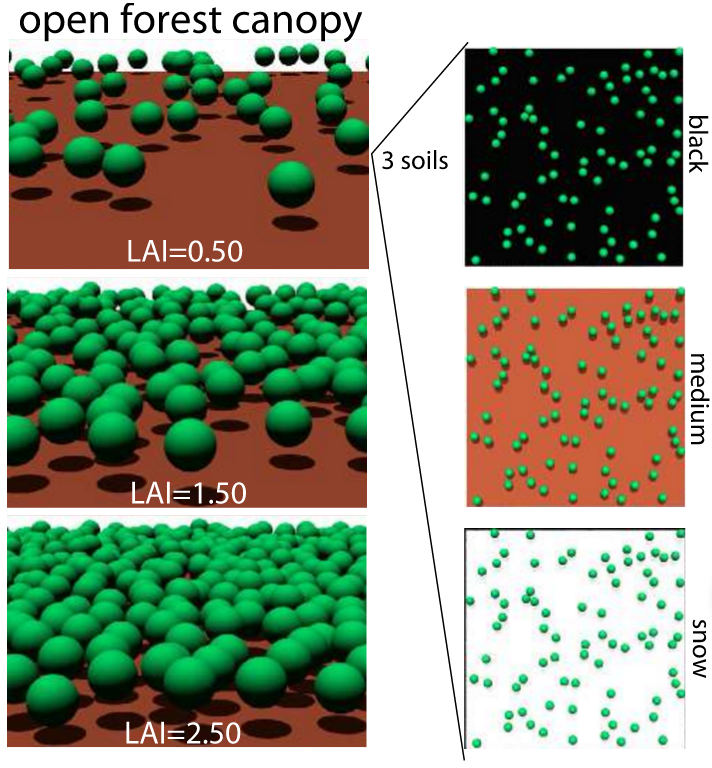
\includegraphics[width=1.0\textwidth]{/home/mn811042/Thesis/chapter2/figures/Figure_8_rami4pilps_2011.png}
\caption{Graphical representation of the open forest canopy environments used in RAMI4PILPS. The images on the left represent three different canopy structures and three different background brightness (from \citet{Widlowski2011}).}
\label{f:rami}
\end{figure}

Experiments like RAMI4PILPS allow an assessment of the implications on radiative balance due to a choice of a particular canopy radiative transfer scheme, and it is important when decisions on further LSMs development need to be made with limited resources \citep{loew2014}.

While model evaluation studies point out to deviations of model results compared to other models and somehow assess the skills of mathematical schemes \citep{Hagemann2013}, they typically do not provide an assessment of potential impacts of the observed model deficits.

The structure factor parameterisation \citep{pinty2006} seems to have great potentiality to account for canopy structural effects on radiative transfer schemes in LSMs, for several reasons highlighted before, whereas the main novelty is a function of zenith angle, so, it does take into account the variation of vegetation clumping for different Sun/observation geometries.
In order to evaluate a parameterisation in vegetation canopies radiative transfer schemes, as the structure factor, for example, it is therefore necessary to address and assess, at least three major points regarding the potentialities and applicability of the proposition: 
\begin{enumerate}[(i)]
\item to address how capable a parameterisation is in reproduce, or at least largely agree, with canopy radiative transfer formulations of more complex and accurate state-of-the-art 3D radiative transfer models, in order to simulate consistently canopy absorptance, reflectance and transmittance of idealised reference cases; and to assess at which conditions the used canopy radiative transfer schemes with  their parameterisations might lead to major biases in the radiative balance estimates.
\item to address the parameterisation with observed data, or at least, to propose applicable methods for acquisition and validation of the parameterisation, and its direct impacts. As an example, the structure factor is mainly quoted as being an index to be acquired at the satellite pixel level \citep{Pinty2004}, which varies, regarding resolution, between different satellite products. However, regarding this method, there is no theoretical limitation in acquiring the structure factor parameters from other area dimensions, or other sources of data, i.e., non-satellite. This point however needs to be further explored.
\item importantly and most of the time lacking in typical parameterisations proposals is the assessment of potential indirect implications. In this case, indirect implications could be interpreted as differences in carbon productivity estimates, or albedo-induced radiative forcings caused by using different parameterisations, instead of not using it.
\end{enumerate}

In the original work, \citet{pinty2006} evaluated the impact of aerosol optical depth on fraction of absorbed PAR (fAPAR) for different canopy structures.  
A direct replacement of 1D canopy radiative transfer schemes by more complex ones  in LSMs is not foreseeable in the near future as the required canopy structural information required for 3D models is not available as prognostic variables from LSMs, and because of much higher computational costs of these models \citep{loew2014}. Parameterisations, however, aim to contour this problem.
Those points should really be considered when analysing the impacts of parameterisations, that account for vegetation structural in canopy radiative transfer schemes in LSMs. Potential impacts of any parameterisation can only be identified only once the target is clearly defined and accurate reference solutions (modelled or observed) are available. Modelling evaluation studies can determine the urgency of new developments to improve relevant model formulations \citep{Widlowski2013}.

Complete and accurate data sets are also required to properly evaluate and develop canopy radiative transfer parameterisations. Several large scale studies were develop in order to improve the understanding of exchanges of energy, water and carbon between the atmosphere and the land-surface, and their controlling processes of the physical climate system. 

As an example of these large field campaigns used to evaluate parameterisations \citep{Kucharik1999;pinty2006}, BOREAS was initiated as a large-scale international investigation of the Canadian boreal forest. The primary goal of BOREAS was to acquire data needed to improve climate models predictions of global change effects, particularly focused on temperature and precipitation differences associated to global warming, as well as giving a better description of atmosphere-biosphere interaction processes \citep{Sellers1997}. From 1993 to 1997, with two series of intensive field campaigns in 1994 and 1996, the experiment was designed to connect a wide range of spatial scales, because a number of important processes could only be studied at very small spatial scale, as few links between radiative transfer, vegetation structure, energy partitioning, and photosynthesis. BOREAS was conducted mainly for the scientific need to fill theoretical, methodological, and observational gaps on mass and energy exchanges between the atmosphere over the boreal forest ecosystem. 

One of the aims of BOREAS was to improve and validate parameterisations, and to enhance methods for deriving parameters from satellite observations. The design and implementation of BOREAS combined allometry, destructive, and optical methods to create ground estimates of LAI, canopy structure, and fAPAR by the vegetation canopy within flux towers. These large data sets led researchers to improve ecophysiological measurements, to develop new methods of data acquiring, and detailed land-surface modelling. 

For example, \citet{Chen1997} found that a manufactured LAI instrument (LAI-2000) underestimated the destructive sample estimates of LAI, because its algorithm assumed a spatially random distribution of leaves to compute LAI as a function of canopy gap fraction. This finding confirmed the importance of vegetation canopy structure in boreal forests and highlighted the difficulties with ground characterisation of biophysical variables. 

Another important novel measuring approach with BOREAS was the combination of a large number of measurements (hemispherical photograph, stand mapping, destructive sampling and modelling), in order to characterise the canopy architecture for boreal forests \citep{Fournier1997}. Stand level field data acquisition is important to input tree-based 3D models, which can fill theoretical gaps between 1D models and actual ecosystems \citep{Widlowski2011}.

The theoretical and observational progress in biogeochemical and atmospheric sciences achieved with BOREAS was unprecedented, not just because of the importance of the boreal forest ecosystem, or the novelty of such a complex experiment, but also the size of the study sites (100 x 50 km), the wide range of study areas (airborne fluxes and meteorology, hydrology, remote sensing, terrestrial ecology), and the large amount of collected data (274 data sets).

Others large-scale experiments were conducted in different regions, or proportions, for example, the First ISLSCP (International Satellite Land Surface Climatology Project) Field Experiment (FIFE) project conducted in the Konza Prairie in Kansas, USA, from 1987 to 1989, within 15 x 15 km area of grassland \citep{Hall1995}; or the Large-Scale Biosphere-Atmosphere Experiment in Amazonia (LBA) conducted from 1995 to 2005 with sparse research areas all over the Amazon region, focused on carbon storage, nutrient dynamics, trace gas fluxes for the tropical rainforest. 
Going into the direction of increase the number of ecosystem structural studies, the National Ecological Observatory Network (NEON) is the first continental scale ecological observatory with airborne remote sensing of vegetation canopy biochemistry and structure \citep{Kampe2010}. Still under construction, the NEON database will provide a robust material to develop land surface studies relating 3D canopy structure and atmosphere-biosphere exchanges of mass and energy. Few other studies have used data from airborne-LiDAR \citep{Chen2008,Kobayashi2012}, which estimates the distribution of plant canopies, as well as sub-canopy topography, providing high-resolution mapping of vegetation height, cover, and canopy structure, but they are still very temporal and spatially limited. 

The importance of addressing canopy structure in fieldwork observations is greatly appreciated by the scientific community. There are several distinct methods to obtain structural patterns from vegetation with their specific qualities and limitations. For example, satellite observations are a valid tool to estimate biogephysical parameters from vegetation over very large areas, usually the whole globe. However, the resolution of these variables are limited to the satellite pixels, which are usually not directly comparable to measurements acquired in-situ. 
In the case of clumping index, \citep{Chen2005} used the bidirectional reflectance distribution function (BRDF) of vegetated land surfaces to extract vegetation structural information globally, using multi-angular data from the POLDER instrument. For the first time, a global clumping index map was derived assisted by a geometrical optical model. However, the clumping index map presented by the author has several limitations, as low spatial resolution (7 km resolution), topographic effects, and a lack of evaluation with field measurements. Later on, further studies from the same research group improved and validated the global clumping index map with in-situ observations \citep{Pisek2010}.

Using the same type of data (BRDFs), \citet{He2012} derived for the first time a global clumping index map at 500 m resolution from MODIS (Moderate Resolution Imaging Spectroradiometer). However, MODIS-derived clumping index map was found to be consistently lower than available ground data, and no zenith angular dependency.

Following the same research questions and deriving a clumping index map from MISR data \citep{Pisek2013}, \citet{Pisek2015} developed a comparison study between all available satellite based clumping index products and in-situ observations. Among their main conclusions, the authors pointed out for the fact that the MODIS clumping index map \citep{He2012} with its spatial resolution at 500 m compared to 6 km from POLDER might be more suitable for use in LSMs given the spatial resolution, and that correct land cover information (broadleaf vs. needle-leaf) is crucial for retrieving accurate clumping index values. Furthermore, satellite sensors cannot provide correct clumping index estimates over areas with insufficient vegetation coverage ($<$ 25\%), i.e., sparse canopies.
One way to acquire information about clumping index without the satellite limitation is by using optical field instruments, particularly digital hemispherical photographs. Photographs provide indispensable advantages on simultaneous acquisition of gap fraction in multiple directions, permanent recordings and spatial discrimination leading to the calculation of foliage clumping \citep{Gonsamo2009}. 

In the particular case of the structure factor, that accounts for zenith variations of clumping index, digital hemispherical photographs are more indicated than satellite measurements. 
In summary, it is clear the growth interest of the research community in develop, test and apply methods to address canopy vegetation structure in a feasible way affecting the radiation partitioning, especially to be directly used in LSMs and allow improvements in weather forecast and climate predictions.
However, further evaluations have to be addressed in previously proposed parameterisations, especially regarding their ability in reproduce more complex models results, and actually reproduce what is measured in the real world. 

Furthermore, the indirect impacts of parameterisations on applicable knowledge improvements is necessary, and opens a new horizon to be scientifically explored. 




